\clearpage 
\section{Further details on the MC template method}
\label{app_mc_template}
	
In order to validate the fitting machinery, we performed pseudo-experiments where the toy data is obtained 
by randomly sampling the summed contribution from the six categories according to a Poisson distribution. 
Pull plots are obtained for each fake rate as shown in Figure \ref{f:pull_test}. 
Overall, the mean is consistent with zero and the standard deviation is close to unity as expected. 

\begin{figure}[htb]
 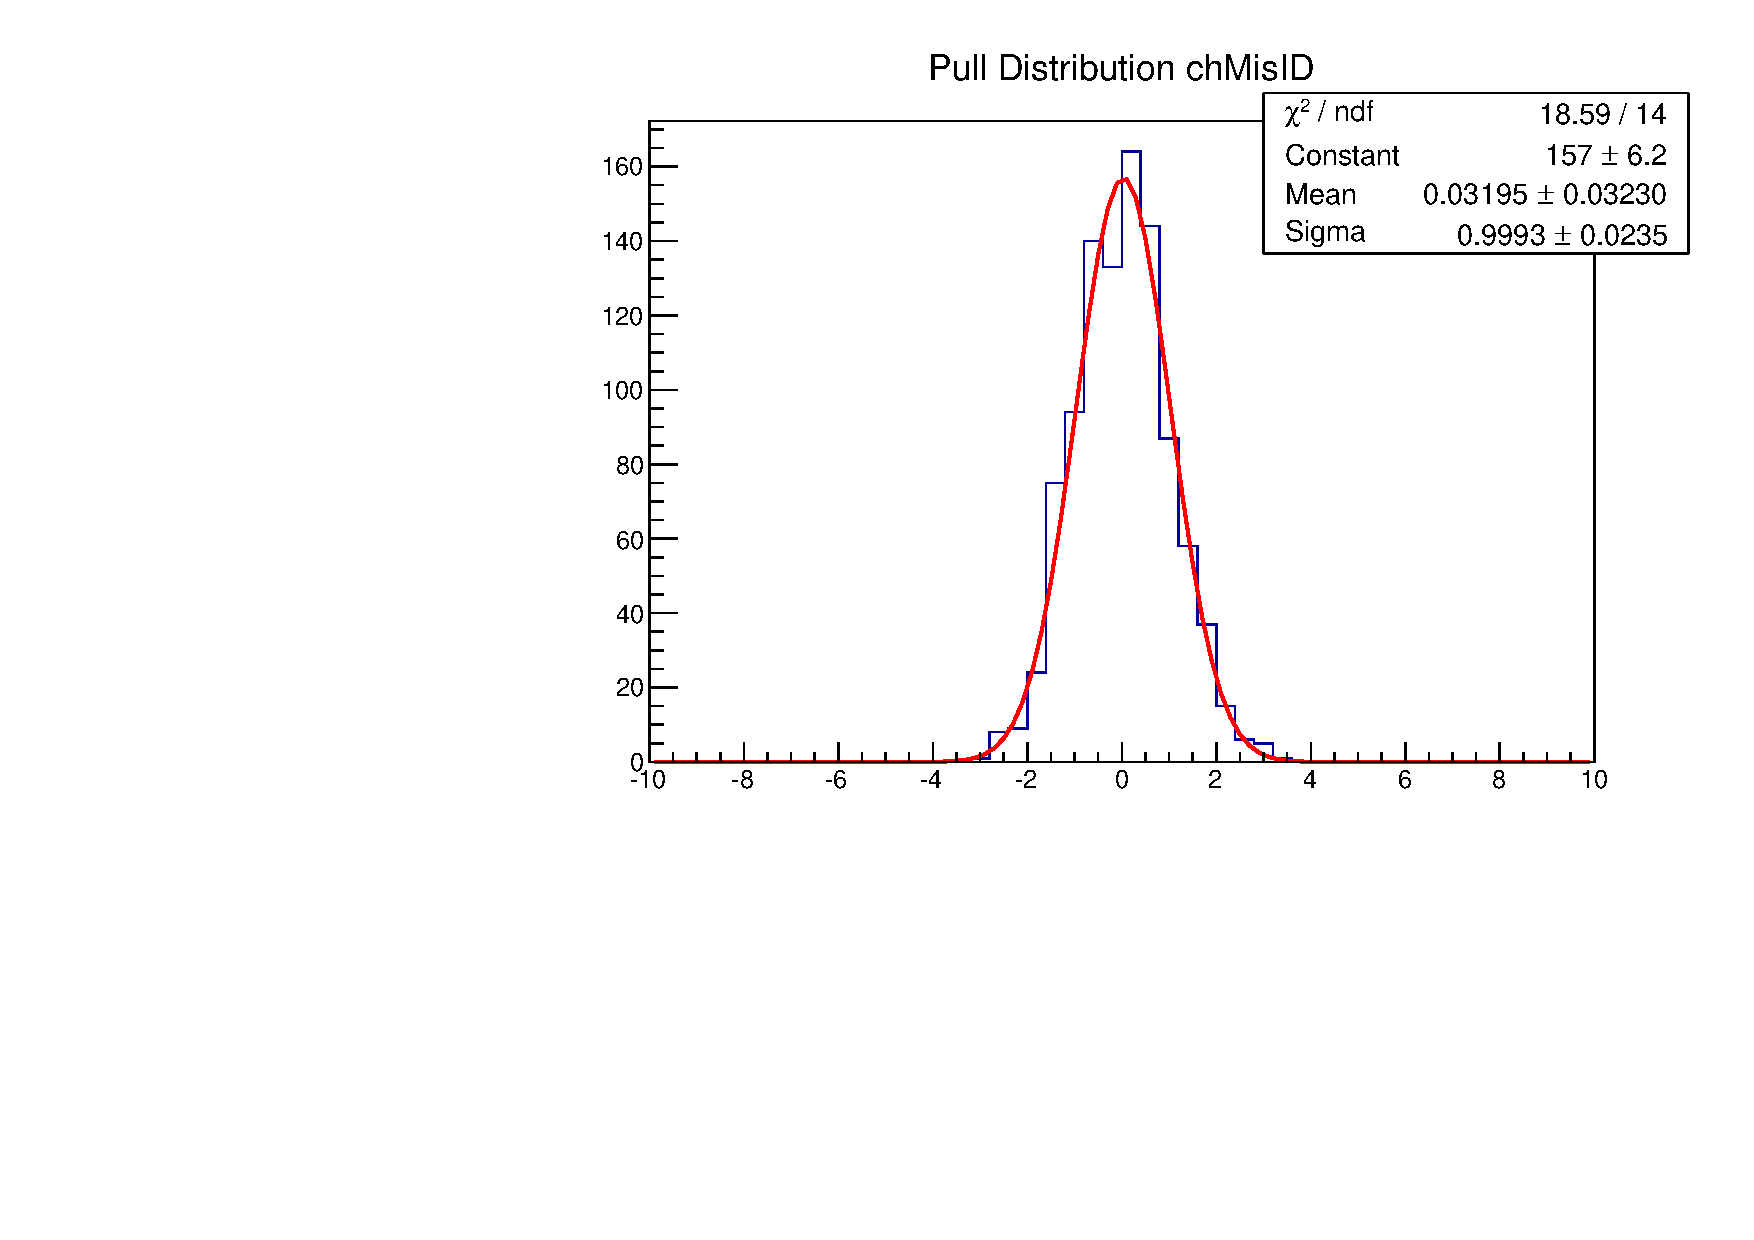
\includegraphics[width=.33\textwidth]{FIGURES/bckg_MC/Pull/L10ifb/chMisID.pdf}
  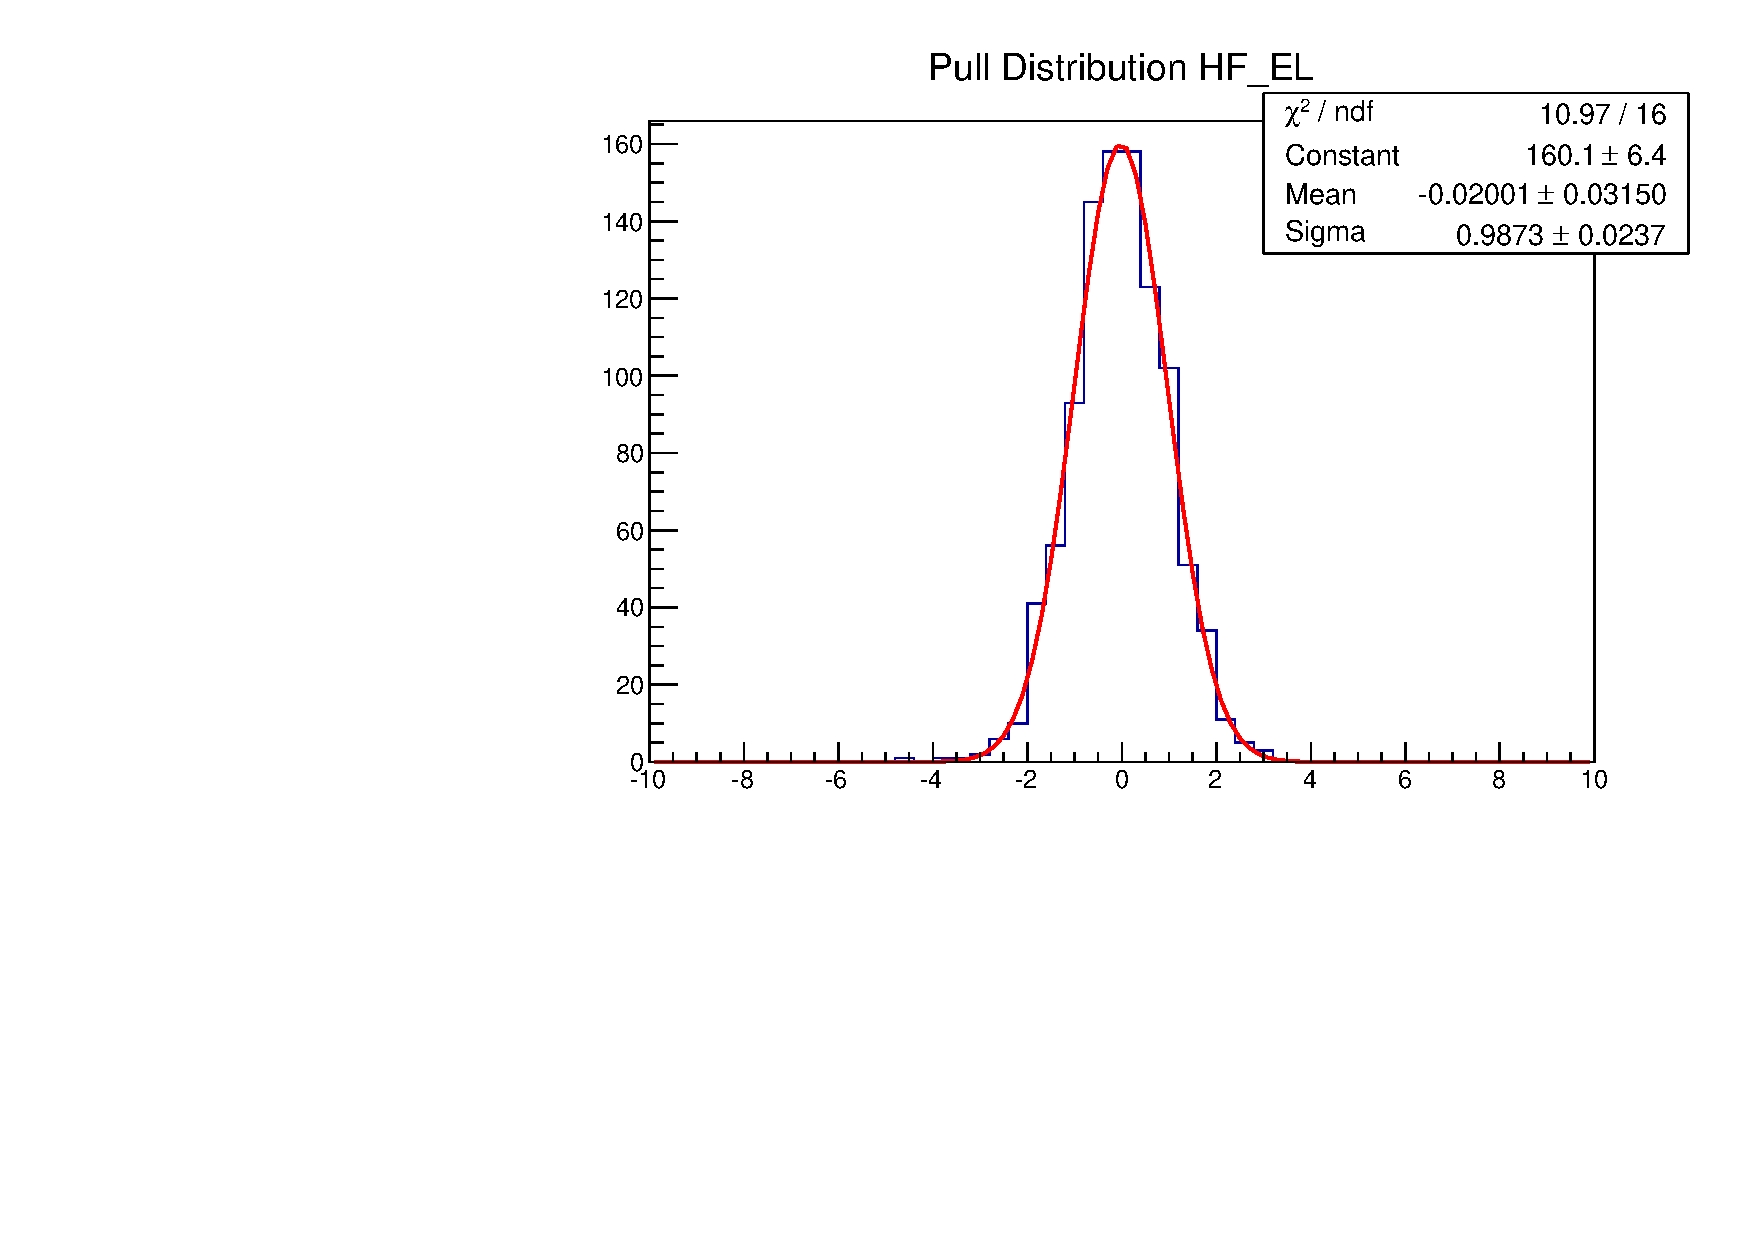
\includegraphics[width=.33\textwidth]{FIGURES/bckg_MC/Pull/L10ifb/hf_el.pdf}
  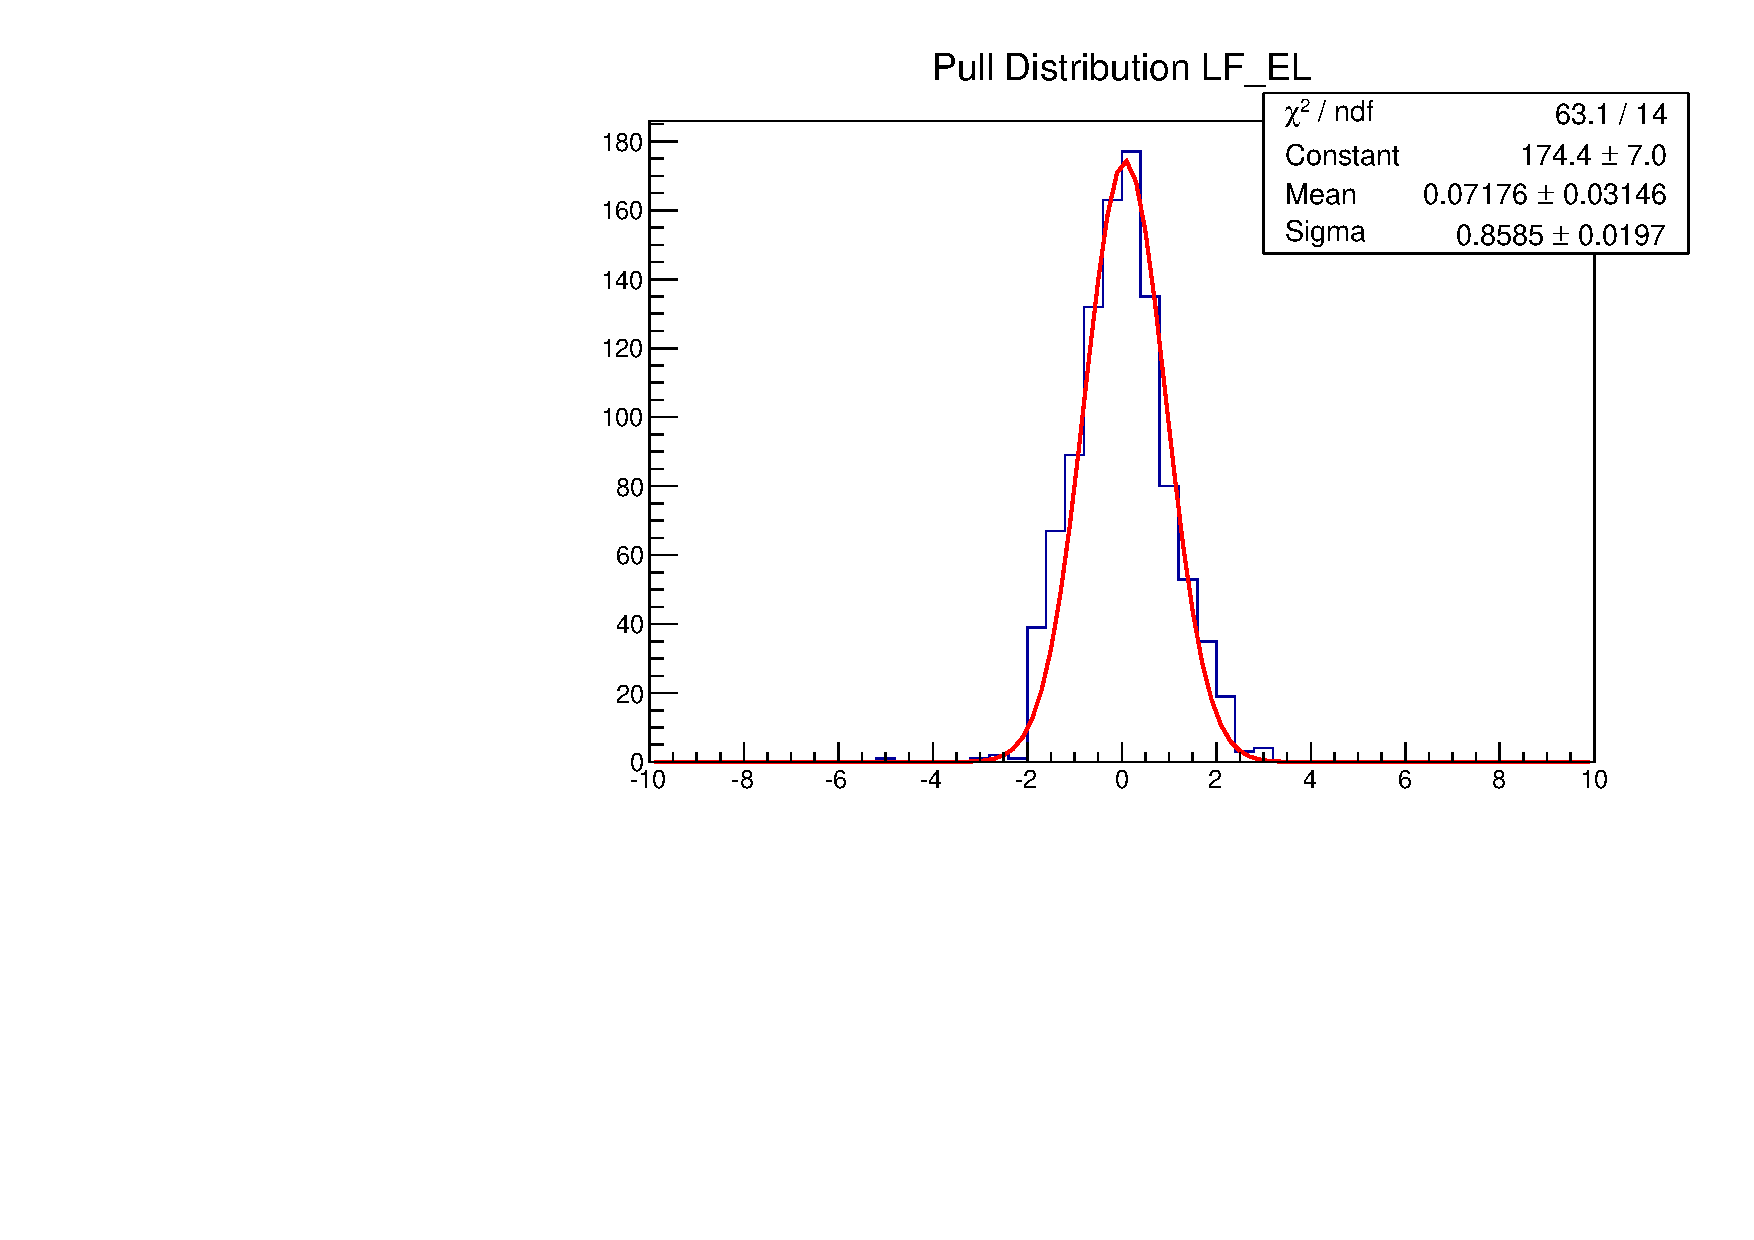
\includegraphics[width=.33\textwidth]{FIGURES/bckg_MC/Pull/L10ifb/lf_el.pdf} \\
  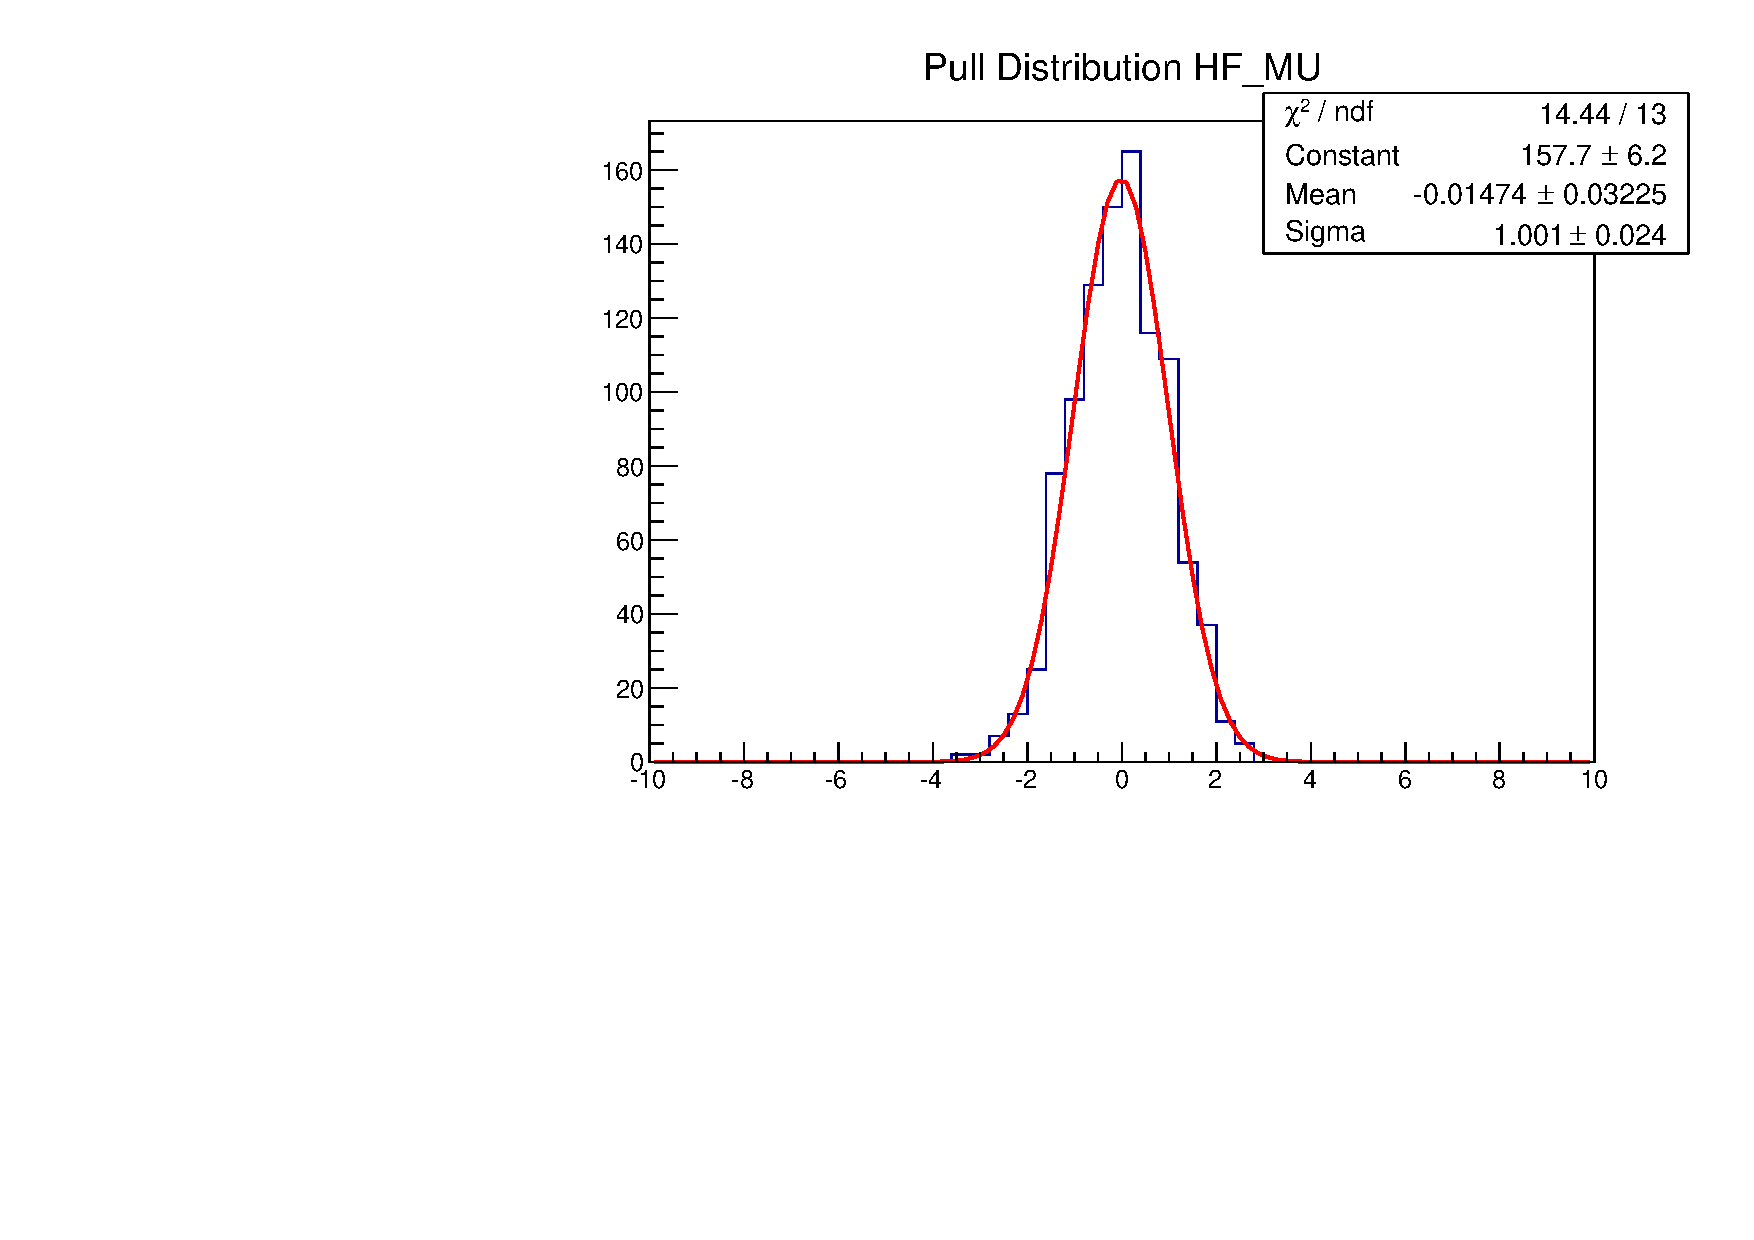
\includegraphics[width=.33\textwidth]{FIGURES/bckg_MC/Pull/L10ifb/hf_mu.pdf}
  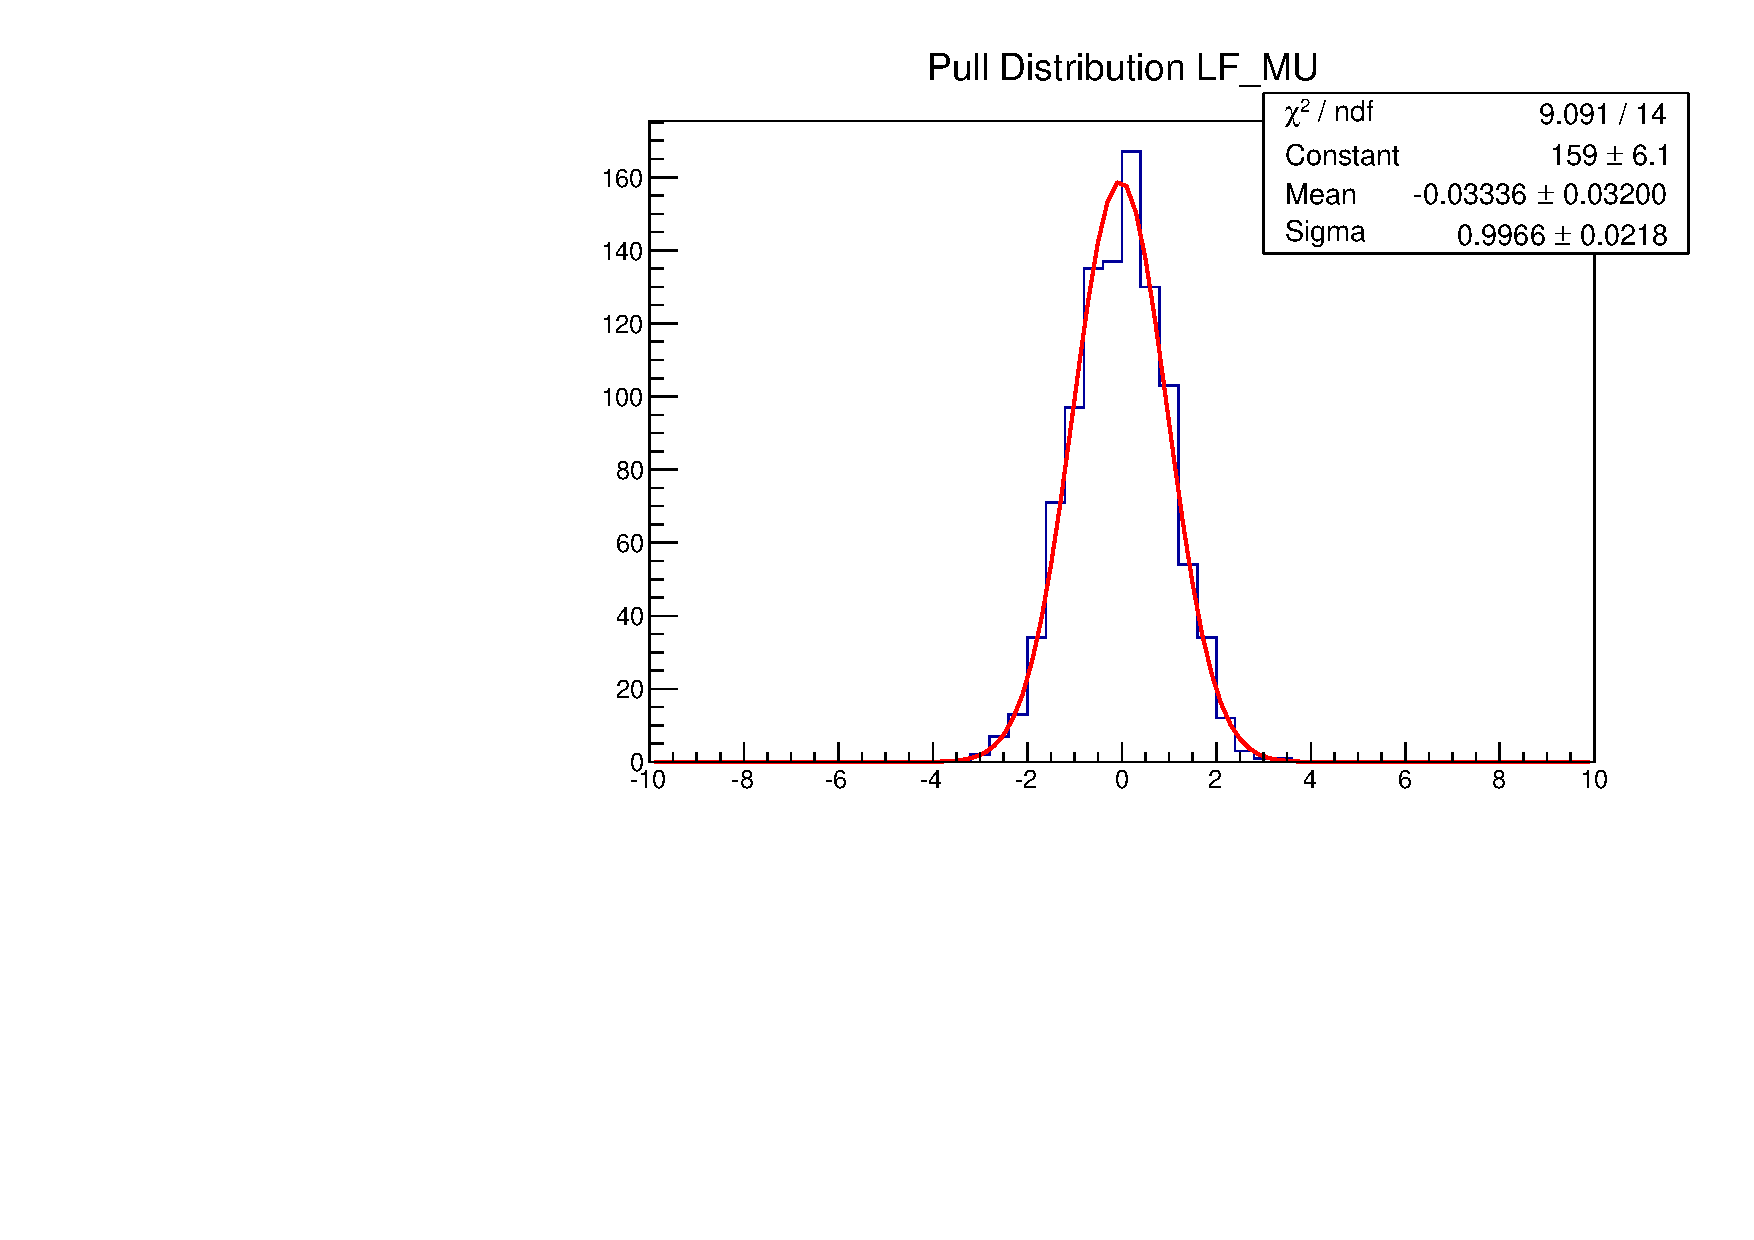
\includegraphics[width=.33\textwidth]{FIGURES/bckg_MC/Pull/L10ifb/lf_mu.pdf} \\
\caption{Pull tests for the correction factors using toy data.
\label{f:pull_test}
}
\end{figure}


In our classification, we assumed that the $b$-tagging requirement only affects the rate of leptons coming from $b$-hadrons. 
As a sanity check of this assumption, we also include fake leptons coming from c-hadron decays in HF 
with the leptons coming from $b$-hadrons and re-do the fit. 
The comparison is shown in Table~\ref{t:compare_b_bc} using pseudo-data which shows that there is a negligeable effect in including $c$-jet induced fakes. 

 \begin{table}[!htb]
  \caption{The fake-rate and charge flip corrections obtained in the cases where fakes from c-hadrons are categorized separate from fakes from $b$-hadrons and  when they are categorized in the same category. A negligeable effect is observed. The MC templates are normalized to 2 \ifb of integrated luminosity.
  \label{t:compare_b_bc}}
%\scalebox{.8}{
\centering
    \begin{tabular}{|c|c|c|}
      \hline
      Category & $b$-hadrons & $b-$ or $c-$hadrons \\
      \hline
      Charge Flip   &   1.02 $\pm$ 0.11  & 1.02  $\pm$  0.11 \\
      EL HF     &   0.99 $\pm$ 0.85  & 1.00  $\pm$  0.83 \\
      EL LF     &   0.69 $\pm$ 0.84  & 0.69  $\pm$  0.82 \\
      MU HF     &   1.01 $\pm$ 0.28  & 0.97  $\pm$  0.24 \\
      MU LF     &   0.85 $\pm$ 0.84  & 0.92  $\pm$  0.93 \\
      \hline
    \end{tabular}
%}
 \end{table}


